\chapter{Anforderungen}\index{Anforderungen}
Als Beispiel nehmen wir wieder unser bekanntes Blackboard. Das Blackboard hat von uns vier Anforderungen bekommen. Diese werden in funktionale und nichtfunktionale Anforderungen unterteilt. Dies ist eine g�ngige Unterteilung in der Softwareentwicklung.\\
Funktionale Anforderungen beschreiben die Eigenschaften einer Funktion, also was das Produkt tun soll. Nichtfunktionale Anforderungen beschreiben Eigenschaften eines Produktes, also wie das Produkt etwas tun soll.\\
Bei unserem Blackboard haben wir die drei funktionalen Anforderungen \textit{Notiz hinzuf�gen}, \textit{Notiz bearbeiten}, \textit{Notiz l�schen} und die nichtfunktionale Anforderung \textit{Desgin}. Betrachten wir uns die funktionale Anforderung \textit{Notiz hinzuf�gen} in Abb. \ref{fig:LastenheftAnforderungF1}.
\begin{figure}[H]
\centering
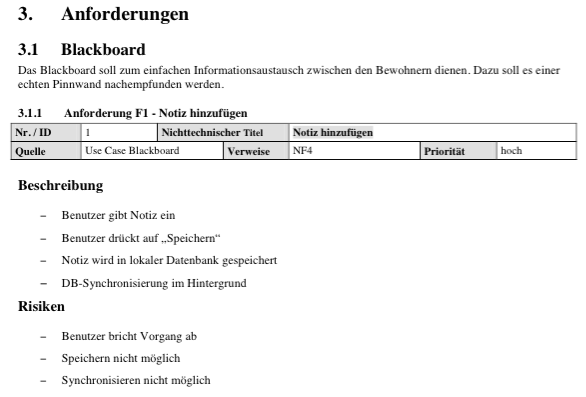
\includegraphics[width=\linewidth]{images/vorgehensweise/lastenheft/LastenheftAnforderungenBlackBoard.png}
\caption{Anforderung F1 - Notiz hinzuf�gen (Blackboard)}
\label{fig:LastenheftAnforderungF1}
\end{figure}